\begin{frame}{SeaThru}
    \centering
    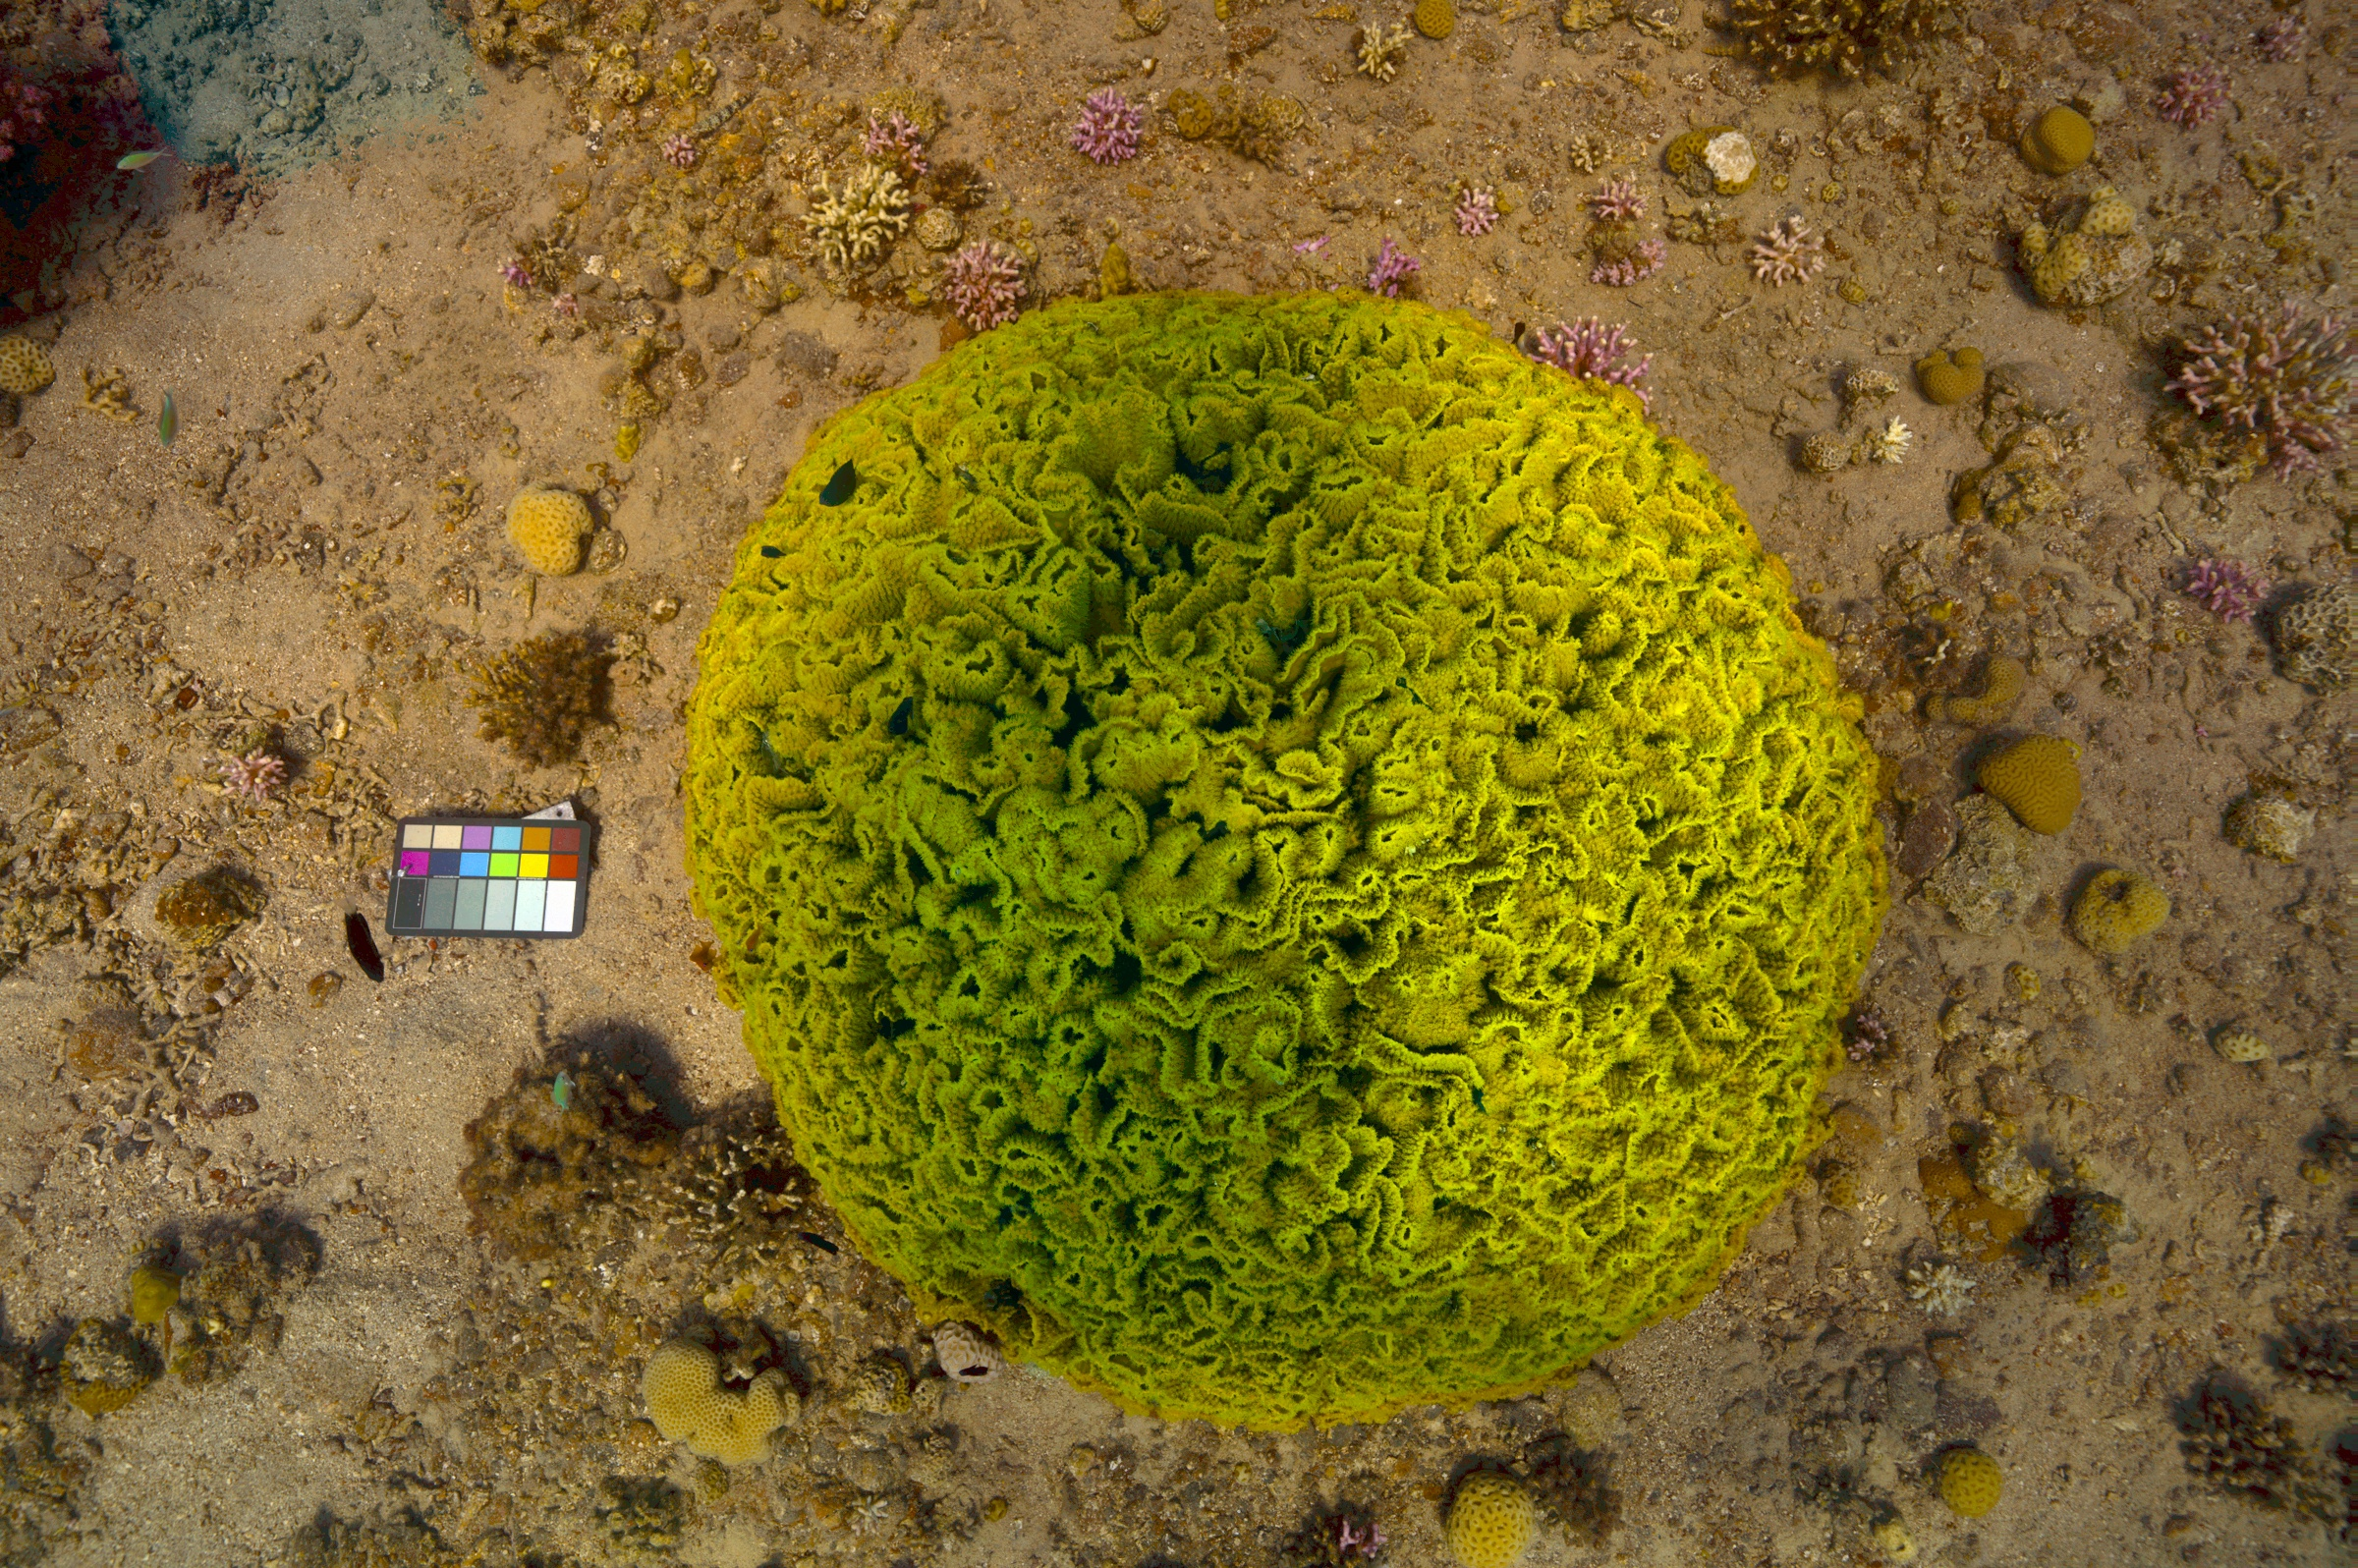
\includegraphics[height=0.7\textheight,width=0.7\textwidth,keepaspectratio]{images/crutchfield_final.jpg}
\end{frame}

\begin{frame}{SeaThru}
    \centering
    \includegraphics[height=0.7\textheight,width=0.7\textwidth,keepaspectratio]{images/crutchfield2_final.png}
\end{frame}

\begin{frame}{SeaThru}
    \centering
    \includegraphics[height=0.7\textheight,width=0.7\textwidth,keepaspectratio]{images/crutchfield_perry_final.png}
\end{frame}

\begin{frame}{Attenuation Map Optimization}
    $$min_{a,b,c,d} || z - \frac{-\log{\hat{E}_c}}{ae^{bz} + ce^{dz}} ||$$
    subject to
    $$a \geq 0; b \leq 0; c \geq 0; d \leq 0$$
\end{frame}

\begin{frame}{Non Linear Least Squares Fitting}
    $$\hat{B}_c = B_c^{\infty}(1-e^{-\Beta_c^B z})+J'_c e^{-\Beta_c^{D' z}$$
    subject to
    $$0 \leq B^\infty_c \geq 1; 0 \leq \Beta_c^B \geq B; 0 \leq J'_c \geq 1; 0 \leq \Beta_c^{D'}$$
\end{frame}

% Slides for 2025-01-13
% To create a slide, use the following:
% \begin{frame}{TITLE}
%     BODY
% \end{frame}

% To create a slide with a bullet list, use the following:
% \begin{frame}{TITLE}
%     \begin{itemize}
%         \item ITEM 1
%         \item ITEM 2
%     \end{itemize}    
% \end{frame}

% To create a slide with numbered list, use the following:
% \begin{frame}{TITLE}
%     \begin{enumerate}
%         \item ITEM 1
%         \item ITEM 2
%     \end{enumerate}
% \end{frame}

% To create a slide with a graphic:
% 1. Add the graphic to this folder (named picture.png)
% 2. Use the following:
% \begin{frame}{TITLE}
%     \centering
%     \includegraphics[height=0.7\textheight,width=0.7\textwidth,keepaspectratio]{picture.png}
% \end{frame}

% To create a slide with two columns, use the following:
% \begin{frame}{TITLE}
%     \begin{columns}
%         \begin{column}{0.5\textwidth}
%             COLUMN 1 BODY
%         \end{column}
%         \begin{column}{0.5\textwidth}
%             COLUMN 2 BODY
%         \end{column}
%     \end{columns}
% \end{frame}
